% --------------------------------------------------------------
% This is all preamble stuff that you don't have to worry about.
% Head down to where it says "Start here"
% --------------------------------------------------------------
 
\documentclass[12pt]{article}
 \listfiles
\usepackage[margin=1in]{geometry} 
\usepackage{amsmath,amsthm,amssymb,mathtools}
\usepackage{float}
\usepackage{graphicx}
\usepackage{cancel}
\usepackage{tikz}
\usepackage{xcolor}
\usepackage{bm}
\usepackage{tikz}
\usepackage{bm}
\usepackage{cancel}
\usepackage{filecontents}
\usepackage{algorithm}
\usepackage{algpseudocode} % loads algorithmicx

\usepackage{pgfplots}
%\pgfplotsset{compat=1.10}
\usetikzlibrary{intersections}
%\usepgfplotslibrary{fillbetween}

\newcommand{\N}{\mathbb{N}}
\newcommand{\Z}{\mathbb{Z}}
\newcommand{\sign}[1]{\text{sign}(#1)}
\newcommand{\abs}[1]{\left| #1 \right|}
\newcommand{\BigO}[1]{\mathcal{O}\left( #1 \right)}
\newcommand{\LittleO}[1]{\mathcal{o}\left( #1 \right)}
\renewcommand{\Pr}[1]{\text{Pr}[ #1 ]}
\newcommand{\norm}[1]{\left|\left| #1 \right|\right|}
\newcommand{\inner}[2]{\left< #1 , #2\right>}
\newcommand{\R}{\mathbb{R}}
\newcommand{\grad}{\nabla}
\renewcommand{\P}[1]{\left( #1 \right)}
\newcommand{\B}[1]{\left[ #1 \right]}
\def\layersep{2.5cm}
 
\newenvironment{theorem}[2][Theorem]{\begin{trivlist}
\item[\hskip \labelsep {\bfseries #1}\hskip \labelsep {\bfseries #2.}]}{\end{trivlist}}
\newenvironment{lemma}[2][Lemma]{\begin{trivlist}
\item[\hskip \labelsep {\bfseries #1}\hskip \labelsep {\bfseries #2.}]}{\end{trivlist}}
\newenvironment{exercise}[2][Exercise]{\begin{trivlist}
\item[\hskip \labelsep {\bfseries #1}\hskip \labelsep {\bfseries #2.}]}{\end{trivlist}}
\newenvironment{problem}[2][Problem]{\begin{trivlist}
\item[\hskip \labelsep {\bfseries #1}\hskip \labelsep {\bfseries #2.}]}{\end{trivlist}}
\newenvironment{question}[2][Question]{\begin{trivlist}
\item[\hskip \labelsep {\bfseries #1}\hskip \labelsep {\bfseries #2.}]}{\end{trivlist}}
\newenvironment{corollary}[2][Corollary]{\begin{trivlist}
\item[\hskip \labelsep {\bfseries #1}\hskip \labelsep {\bfseries #2.}]}{\end{trivlist}}

%\algrenewcommand{\algorithmiccomment}[1]{\hskip3em$\vartriangleright$ #1}
\algnewcommand\algorithmicinput{\textbf{Input:}}
\algnewcommand\Input{\item[\algorithmicinput]}
\algnewcommand\algorithmicoutput{\textbf{Output:}}
\algnewcommand\Output{\item[\algorithmicoutput]}


\begin{document}
 
% --------------------------------------------------------------
%                         Start here
% --------------------------------------------------------------
 
\title{Homework 3}%replace X with the appropriate number
\author{Christopher Mertin\\ %replace with your name
CS6966: Theory of Machine Learning} %if necessary, replace with your course title
 
\maketitle

\begin{enumerate}
  \setcounter{enumi}{9}
\item Consider the simple experts setting: we have $n$ experts $E_{1}, \ldots, E_{n}$, and each one makes a $0/1$ prediction each morning. Using these predictions, we need to make a prediction each morning, and at the end of the day we get a loss of $0$ if we predicted right, and $1$ if we made a mistake. This goes on for $T$ days.

Consider an algorithm that at every step, goes with the prediction of the ``best'' ({\em i.e.} the one with the least mistakes so far) expert so far. Suppose that ties are broken by picking the expert with a smaller index. Given an example in whcih this strategy can be really bad -- specifically, the number of mistakes made by the algorithm is roughly a factor of $n$ worse than that of the best expert in hindsight. 

{\bf Solution:}

Consider the case where there are only two experts, $\{ E_{1}, E_{2}\}$ such that $E_{1}$ predicts ``0'' on even days and ``1'' on odd, and $E_{2}$ is the opposite in such that it predicts ``1'' on even days and ``0'' on odd.

Imagine we have the scenario where the ``true value'' is 1 if $t \in $ even and 0 if $t \in $ odd. For a simplified example, we can set $T=4$ and build a table of the values to visualize the iterations. In this, $L(E_{i})$ represents the {\em total loss} at that iteration for expert $i$, and $f(t)$ represents the true value.

\begin{table}[H]
\centering
\begin{tabular}{@{}l c c c c | r@{}}
\hline\hline
$t$ & $E_{1}$ & $E_{2}$ & $L(E_{1})$ & $L(E_{2})$ & $f(t)$\\
\hline
1   & 1      &        & 1          &           &   0\\
2   &        & 0      & 1          & 1         &   1\\
3   & 1      &        & 2          & 1         &   0\\
4   &        & 0      & 2          & 2         &   1\\
\hline
\end{tabular}
\end{table}

This can go on to infinity, but we can see that the total loss can be computed asd $\sum_{i}L(E_{i}) = \BigO{n \min_{i}L(E_{i})}$, meaning that for $n$ experts, we're bounded by $n$ times the ``best expert.'' This can be easily seen as each of the experts will have the same value, so with $n$ experts this goes to be $n$ times the loss of the best.

The above example can be extrapolated easily into $n$ experts by simply stating that $E_{i}$ predicts the same as $E_{1}$ if $i \in $ odd and $E_{i}$ predicts the same as $E_{2}$ if $i \in $ even.

\newpage

\item We saw in class a proof that the VC dimension of the class of $n$-node, $m$-edge {\em threshold} neural networks is $\BigO{(m+n)\log(n)}$. Let us give a ``counting'' proof, assuming the weights are binary $(0/1)$. (This is often the power given by VC dimension based proofs -- they can ``handle'' continuous parameters that cause problems for counting arguments).

\begin{enumerate}
  \item Specifically, how many ``network layouts'' can there be with $n$ nodes and $m$ edges? Show that ${n(n-1)/2}\choose{m}$ is an upper bound.

   {\bf Solution:}
   
   We can say that the total number of layouts based on the edges is $m$. We can also say that we can have 1 node with all of the $m$ edges, or we can have up to $n-1$ different combinations with each node getting different number of edges. Therefore, we get the total number of node combinations to be

   \begin{align*}
     \sum_{i=1}^{n-1}i &== \frac{n(n-1)}{2}
     \intertext{Using the {\em binomial coefficient} to get the total number of combinations gives}
     N &= {n(n-1)/2}\choose{m}
     N &= \frac{(n(n-1)/2)!}{m!(m-n(n-1)/2)!}
     \end{align*}

   \item Given a network layout, argue that the number of ``possible networks'' is at most $2^{m}(n+1)^{n}$. 

[{\em Hint:} What can you say about the potential values for the thresholds?]

   {\bf Solution:}

   As it's a threshold neural network, we know that the weights are binary and so therer are $2^{m}$ different combinations of the weights. We can also change the threshold of the nodes to be valid/non-valid. Valid means that it is set to some useful value, non-valid means that the threshold is set to $\infty$ and thus the node cannot be activated. This gives $\sum_{k=0}^{n}{n}\choose{k} n^{k} = (n+1)^{n}$ different combinations of the thresholds for the nodes. We can multiply the two values together to get the total number of ``possible networks,'' giving

\[
   2^{m}(n+1)^{n}
\]

\item Use these to show that the VC dimension of the class of binary-weight, threshold neural networks is $\BigO{(m+n)\log(n)}$.

   {\bf Solution:}

\end{enumerate}

\newpage

\item (Importance of random initialization) Consider a neural network consisting of (resp.) the input layer $x$, hidden layer $y$, hidden layer $z$, followed by the output node $f$. Suppose that all the nodes in all the layers compute a ``standard'' sigmoid. Also suppose that every node in a layer is connected to every node in the next layer ({\em i.e.}, each layer is fully connected).

Now suppose that all the weights are initialized to $0$, and suppose we start performing SGD using backprop, with a fixed learning rate. Show that at every time step, all the edge weights in a layer are equal.

   {\bf Solution:}

The equation for the sigmoid function is

\begin{align*}
  \sigma(\bm{\theta}_{i}) &= \frac{1}{1 + e^{-\bm{\theta}_{i}}}\\
  \intertext{And we can obtain the derivative as}
  \sigma^{\prime}(\bm{\theta}_{i}) &= \frac{1}{\left[1 + e^{\bm{\theta}_{i}} \right]\left[ 1 + e^{-\bm{\theta}_{i}}\right]}
  \intertext{Finally, we can say that the Jacobian/Cost function for the update is defined as}
  J_{\bm{\theta}}(\sigma) &= \text{diag}(\sigma^{\prime}(\bm{\theta}))
\end{align*}

Where the update is performed by multiplying the weight matrix by $J_{\bm{\theta}}(\sigma)$, which would obtain all of the same values in the back propogation step. There is no source of asymmetry between the neurons when they're initialized the same meaning the neural network can't learn.

It's important to note that as all the values are the same, the gradients for each of the independent weights during the back propogation step would also be the same as they all would be starting at the same value and would all have the same gradients.

\newpage

\item Let us consider networks in whcih each node computes a rectified linear (ReLU) function, and show how they can comptue very ``spiky'' functions of the inptue variables. For this exercise, we restrict to one-variable.

\begin{enumerate}
  \item Consider a single input $x$. Show how to compute a ``triangle wave'' using one hidden layer (constant number of nodes) connected to the input, followed by one output $f$. Formally, we should have $f(x) = 0$ for $x \leq 0$, $f(x) = 2x$ for $0 \leq x \leq 1/2$, $f(x) = 2(1-x)$ for $1/2 \leq x \leq 1$, and $f(x) = 0$ for $x \geq 1$. 

[{\em Hint:} Choose the thresholds for the ReLU's appropriately]

   {\bf Solution:}

This can be done with 3 ReLU neurons, all with equal edge weights of 1. The first neuron is defined as the function $\max\{0, 2x\}$ with a threshold of 0, the second is $\max\{0, 2(1-x) - 2x\}$ with a threshold of $1/2$, and the third is defined as $\max\{0, -2(1-x)\}$ with a threshold of 1. This can be shown to work in the figure below, where this was implemented in Python, where 500 random numbers in the range $(-1, 2)$ were generated and run through these ReLU neurons. 

\begin{figure}[H]
\centering
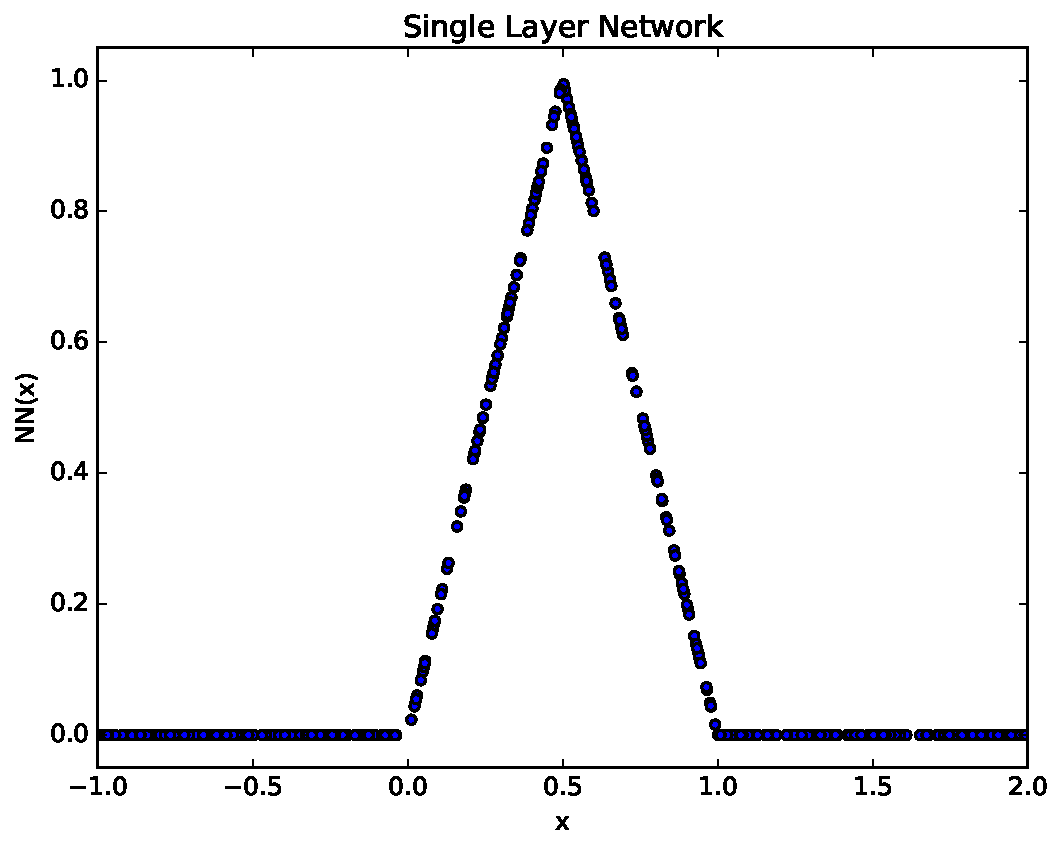
\includegraphics[width=.75\textwidth]{single_layer-13.pdf}
\end{figure}

   {\bf Solution:}

\item What happens if you stack the network on top of itself? (Describe the function obtained). 

[Formally, this means the output of the network you constructed above is fed as the input to an identical network, and we are interested in the final output function.]

   {\bf Solution:}

In doing the above, you get a triangle function again, except all the values are now in the range $(0, 1)$. This can be seen in the figure below, where the results of the previous output were refed into the input of the same network.

\begin{figure}[H]
\centering
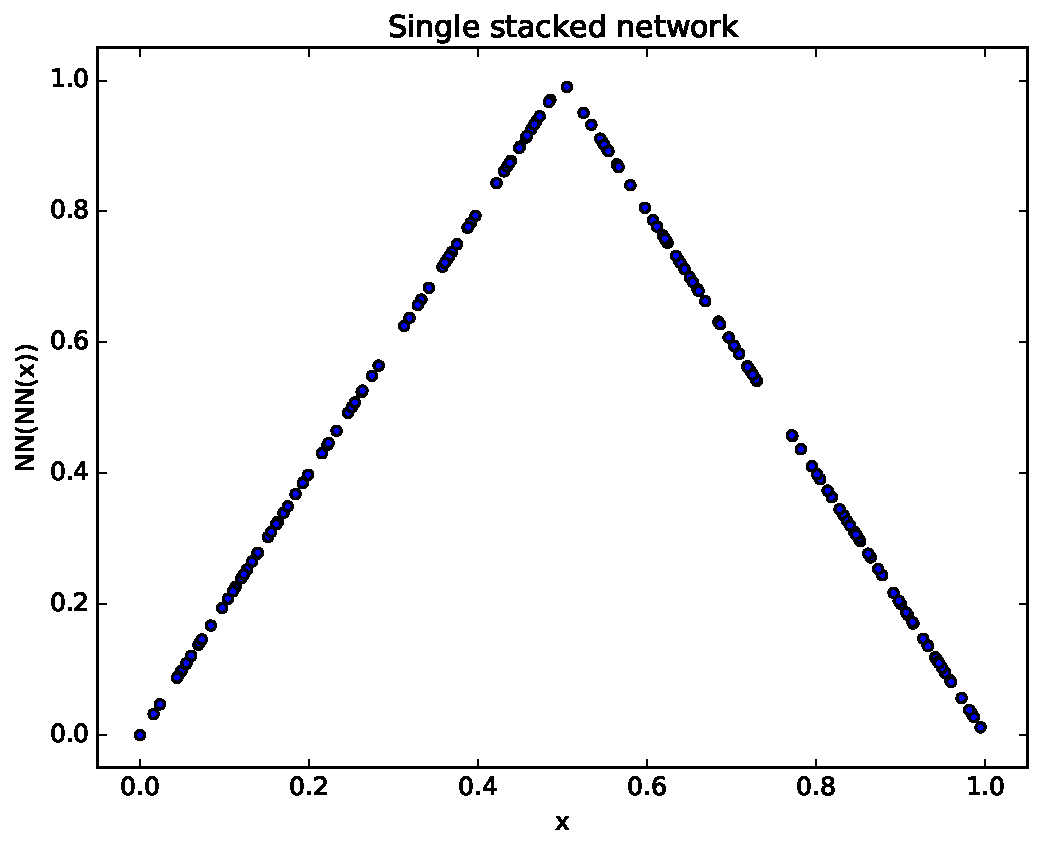
\includegraphics[width=.75\textwidth]{stacked-13.pdf}
\end{figure}

\item Prove that there is a ReLU network with one input variable $x$, $2k + \BigO{1}$ layers, all coefficients and thresholds being constants, that computes a function that has $2^{k}$ ``peaks'' in the interval $[0,1]$.

[The function above can be shown to be impossible to approximate using a small depth ReLU network, without an exponential blow-up in the width.]

   {\bf Solution:}


\end{enumerate}

\newpage

\item In this exercise, we make a simple observatino that width isn't as ``necessary'' as depth. Consider a network in which each node comptues a rectified linar (ReLU) unit -- specifically the function at each node is of the form $\max \{0, a_{1}x_{1} + a_{2}x_{2} + \cdots + a_{m}x_{m} + b\}$, for a node that has inputs $\{ x_{1}, \ldots, x_{m}\}$. Note that different nodes could have different coefficients and offsets ($b$ above is called the offset).

Consider a network with one input $x$, connect to $n$ nodes in a hidden layer, which are in turn connected to the output node, denoted $f$. Show that one can construct a depth $n + \BigO{1}$ network, with just 3 nodes in each layer, to compute the same $f$.

[{\em Hint:} Three nodes allow you to ``carry over'' the input; ReLU's are important for this]

   {\bf Solution:}

The original ``wide'' neural network is of the form

\begin{figure}[H]
\centering
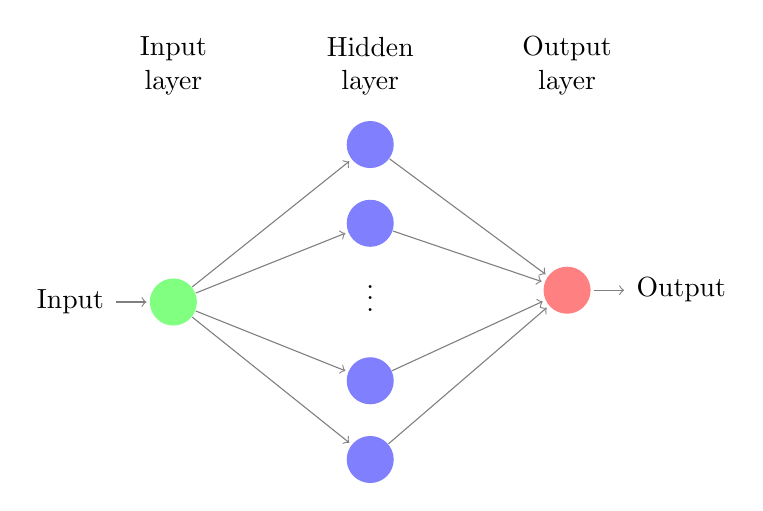
\begin{tikzpicture}[shorten >=1pt,->,draw=black!50, node distance=\layersep]
    \tikzstyle{every pin edge}=[<-,shorten <=1pt]
    \tikzstyle{neuron}=[circle,fill=black!25,minimum size=17pt,inner sep=0pt]
    \tikzstyle{input neuron}=[neuron, fill=green!50];
    \tikzstyle{output neuron}=[neuron, fill=red!50];
    \tikzstyle{hidden neuron}=[neuron, fill=blue!50];
    \tikzstyle{annot} = [text width=4em, text centered]

    % Draw the input layer nodes
    %\foreach \name / \y in {1}%{1,...,4}
    % This is the same as writing \foreach \name / \y in {1/1,2/2,3/3,4/4}
    \node[input neuron, pin=left:Input] (I-1) at (0,-2.5) {};
    \node[] (H-3) at (\layersep, -2.35cm) {$\vdots$};

    % Draw the hidden layer nodes
    \path[yshift=0.5cm]node[hidden neuron] (H-1) at (\layersep, -1 cm) {};
    \path[yshift=0.5cm]node[hidden neuron] (H-2) at (\layersep, -2 cm) {};
    \path[yshift=0.5cm]node[hidden neuron] (H-4) at (\layersep, -4 cm) {};
    \path[yshift=0.5cm]node[hidden neuron] (H-5) at (\layersep, -5 cm) {};
    
    % Draw the output layer node
    \node[output neuron,pin={[pin edge={->}]right:Output}, right of=H-3] (O) {};

    % Connect every node in the input layer with every node in the
    % hidden layer.
    \foreach \source in {1}%,...,4}
        \foreach \dest in {1,2,4,5}%{1,...,5}
            \path (I-\source) edge (H-\dest);

    % Connect every node in the hidden layer with the output layer
    \foreach \source in {1,2,4,5}%{1,...,5}
        \path (H-\source) edge (O);

    % Annotate the layers
    \node[annot,above of=H-1, node distance=1cm] (hl) {Hidden layer};
    \node[annot,left of=hl] {Input layer};
    \node[annot,right of=hl] {Output layer};
\end{tikzpicture}
\end{figure}

This can be changed to a ``deep network'' in the following way. This was made as a depth-4 network, though for a depth $n$ network, the edges between the second and third layer can be repeated networks larger than 4.

\begin{figure}[H]
\centering
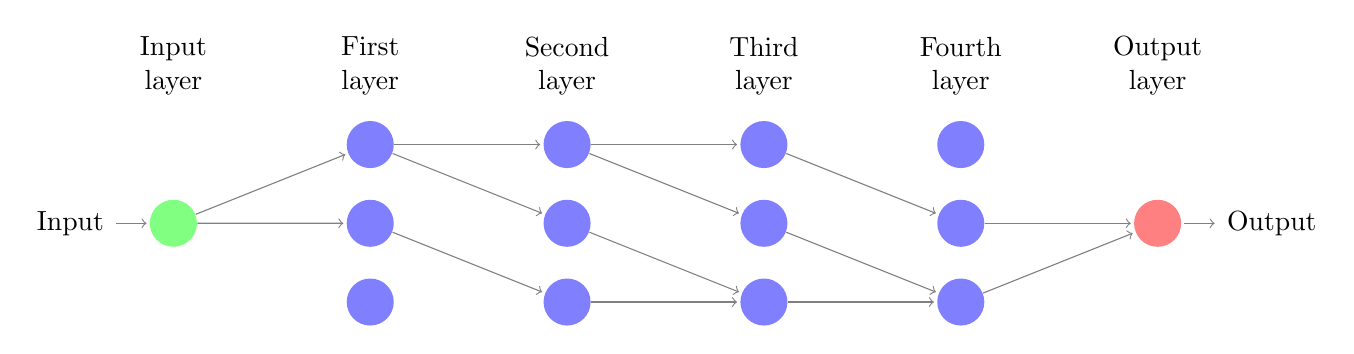
\begin{tikzpicture}[shorten >=1pt,->,draw=black!50, node distance=\layersep]
    \tikzstyle{every pin edge}=[<-,shorten <=1pt]
    \tikzstyle{neuron}=[circle,fill=black!25,minimum size=17pt,inner sep=0pt]
    \tikzstyle{input neuron}=[neuron, fill=green!50];
    \tikzstyle{output neuron}=[neuron, fill=red!50];
    \tikzstyle{hidden neuron}=[neuron, fill=blue!50];
    \tikzstyle{annot} = [text width=4em, text centered]

    % Draw the input layer nodes
    %\foreach \name / \y in {1}%{1,...,4}
    % This is the same as writing \foreach \name / \y in {1/1,2/2,3/3,4/4}
    \node[input neuron, pin=left:Input] (I-1) at (0,-2.5) {};

    % Draw the hidden layer nodes
    \path[yshift=0.5cm]node[hidden neuron] (A-1) at (\layersep, -2 cm) {};
    \path[yshift=0.5cm]node[hidden neuron] (A-2) at (\layersep, -3 cm) {};
    \path[yshift=0.5cm]node[hidden neuron] (A-3) at (\layersep, -4 cm) {};

    \path[yshift=0.5cm]node[hidden neuron] (B-1) at (5, -2 cm) {};
    \path[yshift=0.5cm]node[hidden neuron] (B-2) at (5, -3 cm) {};
    \path[yshift=0.5cm]node[hidden neuron] (B-3) at (5, -4 cm) {};

    \path[yshift=0.5cm]node[hidden neuron] (C-1) at (7.5, -2 cm) {};
    \path[yshift=0.5cm]node[hidden neuron] (C-2) at (7.5, -3 cm) {};
    \path[yshift=0.5cm]node[hidden neuron] (C-3) at (7.5, -4 cm) {};

    \path[yshift=0.5cm]node[hidden neuron] (D-1) at (10, -2 cm) {};
    \path[yshift=0.5cm]node[hidden neuron] (D-2) at (10, -3 cm) {};
    \path[yshift=0.5cm]node[hidden neuron] (D-3) at (10, -4 cm) {};
    
    % Draw the output layer node
    \node[output neuron,pin={[pin edge={->}]right:Output}, right of=D-2] (O) {};

    % Connect every node in the input layer with every node in the
    % hidden layer.
    \foreach \source in {1}%,...,4}
        \foreach \dest in {1,...,2}%{1,...,5}
            \path (I-\source) edge (A-\dest);

    \path (A-1) edge (B-1);
    \path (A-1) edge (B-2);
    \path (A-2) edge (B-3);
    \path (B-1) edge (C-1);
    \path (B-1) edge (C-2);
    \path (B-2) edge (C-3);
    \path (B-3) edge (C-3);
    \path (C-1) edge (D-2);
    \path (C-2) edge (D-3);
    \path (C-3) edge (D-3);

    % Connect every node in the hidden layer with the output layer
    \foreach \source in {2,...,3}%{1,...,5}
        \path (D-\source) edge (O);

    % Annotate the layers
    \node[annot,above of=A-1, node distance=1cm] (hl) {First layer};
    \node[annot,left of=hl] {Input layer};
    \node[annot,right of=hl] (bl) {Second layer};
    \node[annot,right of=bl] (cl) {Third layer};
    \node[annot,right of=cl] (dl) {Fourth layer};
    \node[annot,right of=dl] {Output layer};
\end{tikzpicture}
\end{figure}

In this network, the value of $x$ is fed only into the first two nodes. The task of the first node is simply to pass the value of $x$ through the network, so it will have a weight of $1$. The second node in the layer calculates the weight for that node relative to $x$. This value is passed to the 3rd node of the {\em next layer} which stores the total sum of all the weights, so the weight for the third nodes will be $1$ as well.
\end{enumerate}
 
\end{document}